% tesesusp.cls, v-0.1.0

% Based on 'bntex2ppgsi.cls', 'abntex2.csl' and on USP guidelines to create
% thesis and dissertation documents.
% See <https://www.overleaf.com/project/64f7bdf1641ad4a3a8482800>
% and <https://teses.usp.br/index.php?option=com_content&
%      view=article&id=52&Itemid=67&lang=en>
% to learn more.

\clearpage

% ----------------------------------------------------------------------
% Cover (mandatory)
% ----------------------------------------------------------------------

\imprimircapa

% ----------------------------------------------------------------------
% Title page (mandatory)
% ----------------------------------------------------------------------

%% Avoid usign this page for qualification exams.
\imprimirfolhaderosto*

% % ----------------------------------------------------------------------
% % Cataloging record (mandatory)
% % ----------------------------------------------------------------------
%
% %% Do not use for qualification exams.
% \begin{fichacatalografica}
%  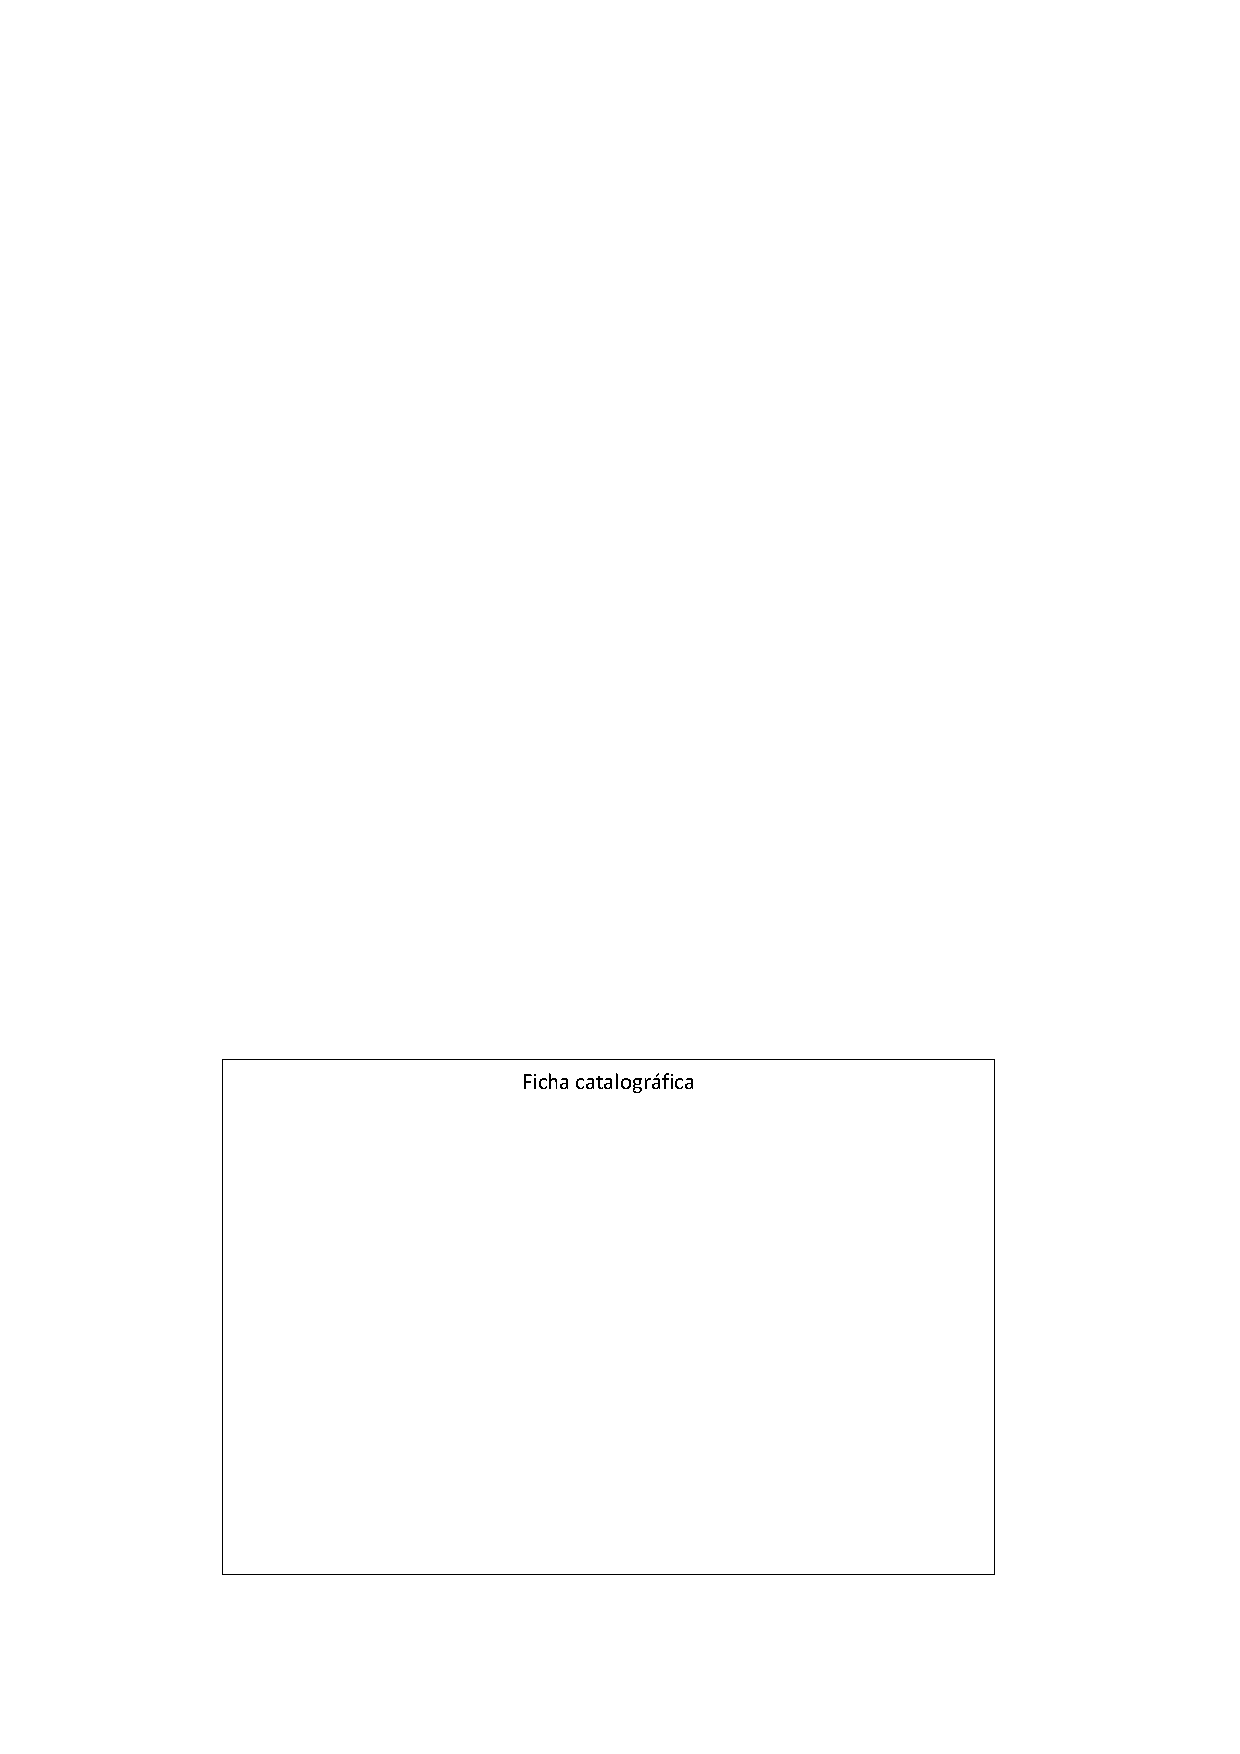
\includepdf{images/fig_ficha_catalografica.pdf}
% \end{fichacatalografica}

% ----------------------------------------------------------------------
% Errata (optional)
% ----------------------------------------------------------------------

\begin{errata}
  \noindent
  % @#$ ERRATA (Render tag - Don't change it)
\end{errata}

% ----------------------------------------------------------------------
% Approval sheet (mandatory)
% ----------------------------------------------------------------------

\begin{folhadeaprovacao}
\noindent
Qualifying exam text by Daniel Vartanian, titled \textbf{``\imprimirtitulo''}, presented to the School of Arts, Sciences and Humanities at the University of São Paulo, as part of the requirements for the degree of Master of Science by the Graduate Program in Modeling Complex Systems (PPG-SCX), in the concentration area of Fundamentals of Complex Systems.

% Dissertation by Daniel Vartanian, titled \textbf{``\imprimirtitulo''}, presented to the School of Arts, Sciences and Humanities at the University of São Paulo, as part of the requirements for the degree of Master of Science by the Graduate Program in Modeling Complex Systems (PPG-SCX), in the concentration area of Fundamentals of Complex Systems.

\vspace*{1.5cm}

\noindent
Approved on \_\_\_\_\_\_\_\_\_\_\_\_\_\_\_\_\_\_\_\_ , \_\_\_\_\_\_\_\_\_\_ .

\vspace*{1.5cm}

\begin{center}
\noindent Examination committee
\end{center}

\vspace*{0.5cm}

\noindent Committee chair:

\vspace*{0.25cm}

\renewcommand{\arraystretch}{2}
\setlength{\arrayrulewidth}{0pt}
\setlength{\tabcolsep}{0pt}
\noindent
\begin{tabular}{m{2cm} P{14cm}}
  Prof. Dr. & \_\_\_\_\_\_\_\_\_\_\_\_\_\_\_\_\_\_\_\_\_\_\_\_\_\_\_\_\_\_\_\_\_\_\_\_\_\_\_\_\_\_\_\_\_\_\_\_\_\_\_\_\_\_\_ \\
  Institution & \_\_\_\_\_\_\_\_\_\_\_\_\_\_\_\_\_\_\_\_\_\_\_\_\_\_\_\_\_\_\_\_\_\_\_\_\_\_\_\_\_\_\_\_\_\_\_\_\_\_\_\_\_\_\_ \\
\end{tabular}

\vspace*{1cm}

\noindent Examiners:

\vspace*{0.25cm}

\noindent
\begin{tabular}{m{2cm} P{14cm}}
  Prof. Dr. & \_\_\_\_\_\_\_\_\_\_\_\_\_\_\_\_\_\_\_\_\_\_\_\_\_\_\_\_\_\_\_\_\_\_\_\_\_\_\_\_\_\_\_\_\_\_\_\_\_\_\_\_\_\_\_ \\
  Institution & \_\_\_\_\_\_\_\_\_\_\_\_\_\_\_\_\_\_\_\_\_\_\_\_\_\_\_\_\_\_\_\_\_\_\_\_\_\_\_\_\_\_\_\_\_\_\_\_\_\_\_\_\_\_\_ \\
  Evaluation & \_\_\_\_\_\_\_\_\_\_\_\_\_\_\_\_\_\_\_\_\_\_\_\_\_\_\_\_\_\_\_\_\_\_\_\_\_\_\_\_\_\_\_\_\_\_\_\_\_\_\_\_\_\_\_ \\
\end{tabular}

\vspace*{0.5cm}

\noindent
\begin{tabular}{m{2cm} P{14cm}}
  Prof. Dr. & \_\_\_\_\_\_\_\_\_\_\_\_\_\_\_\_\_\_\_\_\_\_\_\_\_\_\_\_\_\_\_\_\_\_\_\_\_\_\_\_\_\_\_\_\_\_\_\_\_\_\_\_\_\_\_ \\
  Institution & \_\_\_\_\_\_\_\_\_\_\_\_\_\_\_\_\_\_\_\_\_\_\_\_\_\_\_\_\_\_\_\_\_\_\_\_\_\_\_\_\_\_\_\_\_\_\_\_\_\_\_\_\_\_\_ \\
  Evaluation & \_\_\_\_\_\_\_\_\_\_\_\_\_\_\_\_\_\_\_\_\_\_\_\_\_\_\_\_\_\_\_\_\_\_\_\_\_\_\_\_\_\_\_\_\_\_\_\_\_\_\_\_\_\_\_ \\
\end{tabular}

\vspace*{0.5cm}

\noindent
\begin{tabular}{m{2cm} P{14cm}}
  Prof. Dr. & \_\_\_\_\_\_\_\_\_\_\_\_\_\_\_\_\_\_\_\_\_\_\_\_\_\_\_\_\_\_\_\_\_\_\_\_\_\_\_\_\_\_\_\_\_\_\_\_\_\_\_\_\_\_\_ \\
  Institution & \_\_\_\_\_\_\_\_\_\_\_\_\_\_\_\_\_\_\_\_\_\_\_\_\_\_\_\_\_\_\_\_\_\_\_\_\_\_\_\_\_\_\_\_\_\_\_\_\_\_\_\_\_\_\_ \\
  Evaluation & \_\_\_\_\_\_\_\_\_\_\_\_\_\_\_\_\_\_\_\_\_\_\_\_\_\_\_\_\_\_\_\_\_\_\_\_\_\_\_\_\_\_\_\_\_\_\_\_\_\_\_\_\_\_\_ \\
\end{tabular}
\end{folhadeaprovacao}

% ----------------------------------------------------------------------
% Inscription (optional)
% ----------------------------------------------------------------------

\begin{dedicatoria}
  \vspace*{\fill}
  \centering
  \noindent
  \textit{
  % @#$ INSCRIPTION (Render tag - Don't change it)
  \lipsum[1]
  }
	\vspace*{\fill}
\end{dedicatoria}

% ----------------------------------------------------------------------
% Acknowledgments (optional)
% ----------------------------------------------------------------------

\begin{agradecimentos}
  \noindent
  % @#$ ACKNOWLEDGMENTS (Render tag - Don't change it)
  \lipsum[1]
\end{agradecimentos}

% ----------------------------------------------------------------------
% Epigraph (optional)
% ----------------------------------------------------------------------

%% @theroyalsociety

\begin{epigrafe}
  \vspace*{\fill}
	\begin{flushright}
	  \textit{Nullius in verba} \\
		(The Royal Society, n.d.)
	\end{flushright}
\end{epigrafe}

% ----------------------------------------------------------------------
% Abstract in the vernacular language (mandatory)
% ----------------------------------------------------------------------

\setlength{\absparsep}{18pt}
\begin{resumo}

\begin{flushleft}
% @#$ ABSTRACT-VERNACULAR-CITATION (Render tag - Don't change it)
\end{flushleft}

% @#$ ABSTRACT-VERNACULAR-BODY (Render tag - Don't change it)
\lipsum[1]
\end{resumo}

% ----------------------------------------------------------------------
% Abstract in the foreign language (mandatory)
% ----------------------------------------------------------------------

\begin{resumo}[RESUMO]
\begin{otherlanguage*}{brazil}

\begin{flushleft}
% @#$ ABSTRACT-FOREIGN-CITATION (Render tag - Don't change it)
\end{flushleft}

% @#$ ABSTRACT-FOREIGN-BODY (Render tag - Don't change it)
\lipsum[1]
\end{otherlanguage*}
\end{resumo}

% ----------------------------------------------------------------------
% List of figures (optional)
% ----------------------------------------------------------------------

\renewcommand{\listfigurename}{LIST OF FIGURES}
\pdfbookmark[0]{\listfigurename}{lof}
\listoffigures*
\cleardoublepage

% ----------------------------------------------------------------------
% List of tables (optional)
% ----------------------------------------------------------------------

\renewcommand{\listtablename}{LIST OF TABLES}
\pdfbookmark[0]{\listtablename}{lot}
\listoftables*
\cleardoublepage

% ----------------------------------------------------------------------
% List of abbreviations and acronyms (optional)
% ----------------------------------------------------------------------

\begin{siglas}
  \item[\textbf{\textsubscript{F}}] Subscript indicating a relation with
    work-free days.
  \item[\textbf{\textsubscript{W}}] Subscript indicating a relation with
    workdays.
  \item[\textbf{BT}] Local time of going to bed.
  \item[\textbf{FD}] Number of work-free days per week.
  \item[\textbf{GU}] Local time of getting out of bed.
  \item[\textbf{HO}] Horne \& Ostberg's morningness-eveningness questionnaire
    (same as \emph{MEQ}).
  \item[\textbf{LE}] Light exposure.
  \item[\textbf{LE\textsubscript{week}}] Average weekly light exposure.
  \item[\textbf{MCTQ}] Munich ChronoType Questionnaire.
  \item[\textbf{MCTQ\textsuperscript{PT}}] Portuguese version of the MCTQ.
  \item[\textbf{MEQ}] Morningness-Eveningness Questionnaire.
  \item[\textbf{MSF}] Local time of mid-sleep on work-free days.
  \item[\textbf{MSF\textsubscript{sc}}] Chronotype proxy. The midpoint between
    sleep onset and sleep end on work-free days. A sleep correction
    (\textsubscript{SC}) is made when a possible sleep compensation
    related to a lack of sleep on workdays is identified.
  \item[\textbf{MSW}] Local time of mid-sleep on workdays.
  \item[\textbf{PRC}] Phase response curve.
  \item[\textbf{SD}] Sleep duration.
  \item[\textbf{SD\textsubscript{week}}] Average weekly sleep duration.
  \item[\textbf{SE}] Local time of sleep end.
  \item[\textbf{SI}] ``Sleep inertia''. Despite the name, this abbreviation
    represents the time the respondent takes to get up after sleep end. It
    is used this way by the MCTQ authors.
  \item[\textbf{SJL}] Absolute social jetlag.
  \item[\textbf{SJL\textsubscript{rel}}] Relative social jetlag.
  \item[\textbf{SJL\textsubscript{sc}}] Jankowski's sleep-corrected social
    jetlag.
  \item[\textbf{SJL\textsubscript{sc-rel}}] Jankowski's relative
    sleep-corrected social jetlag.
  \item[\textbf{Sloss\textsubscript{week}}] Weekly sleep loss.
  \item[\textbf{SO}] Local time of sleep onset.
  \item[\textbf{Slat}] Sleep latency or time to fall asleep after preparing to
    sleep on workdays.
  \item[\textbf{SPrep}] Local time of preparing to sleep.
  \item
    \textbf{TBT}: Total time in bed.
  \item[\textbf{WD}] Number of workdays per week.
\end{siglas}

% % ----------------------------------------------------------------------
% % List of symbols (optional)
% % ----------------------------------------------------------------------
%
% \begin{simbolos}
%   \item[$\Gamma$] Gamma
%   \item[$\Lambda$] Lambda
%   \item[$\zeta$] zeta
%   \item[$\in$] In/Belongs
% \end{simbolos}

% ----------------------------------------------------------------------
% Table of contents (mandatory)
% ----------------------------------------------------------------------

\renewcommand{\contentsname}{TABLE OF CONTENTS}
\pdfbookmark[0]{\contentsname}{toc}
% \tableofcontents*
\cleardoublepage
